%%%%%%%%%%%%%%%%%%%%%%%%%%%%%%%%%%%%%%%%%%%%%%%%%%%%%%%%%%%%%%%%
%                                                              %
% LICENSES                                                     %
%                                                              %
%%%%%%%%%%%%%%%%%%%%%%%%%%%%%%%%%%%%%%%%%%%%%%%%%%%%%%%%%%%%%%%%
%                                                              %
% Copyright (C) 2023, Yong Hoon Lee (yhlee@memphis.edu)        %
% This LaTeX template was developed to assist students in      %
% writing their thesis and dissertation. If you find this      %
% resource helpful, you may choose to acknowledge it briefly   %
% in the Acknowledgments section of your document. However,    %
% this is entirely at the author's discretion and is not a     %
% requirement.                                                 %
%                                                              %
% Please note that while this template has been designed to    %
% assist students in writing their thesis or dissertation, it  %
% may not fully conform to the Thesis/Dissertation Guidelines  %
% provided on the Graduate School of the University of Memphis %
% website. It is the responsibility of the individual author   %
% to carefully review and ensure that their document adheres   %
% to the formatting and style requirements outlined in the     %
% guidelines. The author of this template cannot guarantee     %
% full compliance with the guidelines.                         %
%                                                              %
% This work may be distributed and/or modified under the       %
% conditions of the LaTeX Project Public License,              %
% either version 1.3 of this license or (at your option) any   %
% later version. The latest version of this license is in      %
% http://www.latex-project.org/lppl.txt and version 1.3 or     %
% later is part of all distributions of LaTeX version          %
% 2005/12/01 or later.                                         %
% Original `uofm' class package can be obtained from           %
% https://github.com/yonghoonlee/UofM-thesis-template          %
% (Original work directed per requirements of the LPPL)        %
%                                                              %
% This work has the LPPL maintenance status `maintained'.      %
% The Current Maintainer of this work is Yong Hoon Lee.        %
% This work consists of the files abbrev.tex, bibstyle.bst,    %
% glo.tex, main.tex, ref.bib, symb.tex, and uofm.cls.          %
%                                                              %
% The reference style file: bibstyle.bst is adopted from       %
% `elsarticle-num.bst', (C) 2007, 2008, 2009 Elsevier Ltd.,    %
% under the conditions of the LaTeX Project Public License,    %
% either version 1.2 of this license or (at your option) any   %
% later version. http://www.latex-project.org/lppl.txt         %
% Original `elsarticle' package can be obtained from           %
% https://www.ctan.org/pkg/elsarticle                          %
% (Original work directed per requirements of the LPPL)        %
%                                                              %
% The class file: uofm.cls is adopted partially from           %
% `report.cls', (C) 1993-2021 LaTeX Project.,                  %
% under the conditions of the LaTeX Project Public License,    %
% either version 1.3c of this license or (at your option) any  %
% later version. https://www.latex-project.org/lppl.txt        %
% Original `base' kernel of the LaTeX that contains the        %
% `report' package can be obtained from                        %
% https://www.ctan.org/pkg/report                              %
% (Original work directed per requirements of the LPPL)        %
%                                                              %
%%%%%%%%%%%%%%%%%%%%%%%%%%%%%%%%%%%%%%%%%%%%%%%%%%%%%%%%%%%%%%%%
%                                                              %
% DOCUMENT CLASS OPTIONS (default values marked with brackets) %
%                                                              %
%%%%%%%%%%%%%%%%%%%%%%%%%%%%%%%%%%%%%%%%%%%%%%%%%%%%%%%%%%%%%%%%
%                                                              %
% Title page options: [master], doctoral.                      %
%                                                              %
% Font size: 10pt, 11pt, [12pt].                               %
% Smaller than 12pt is not recommended.                        %
%                                                              %
% Section numbering options: secnum, [nosecnum].               %
% UofM does not recommend using the section numbers.           %
% The UofM website states: "Do NOT use a numbering system for  %
% title and subheadings (e.g., 1.1, 1.1.1) unless required by  %
% style manual, refereed journal or approved by student's      %
% committee. If they are numbered, please send justification   %
% with review copy."                                           %
%                                                              %
% Hyphenation: hyphenation, [nohyphenation].                   %
% Generally, raggedright and hyphenation are not working well  %
% if used at the same time.                                    %
%                                                              %
% Binding option: boundcopy, [pdfonly].                        %
% boundcopy option may be used to have 1.5-in left margin,     %
% only if a student wishes to produce bound copies for their   %
% advisor, department, etc.                                    %
% Otherwise, pdfonly option is default that creates standard   %
% 1.0-in left margin.                                          %
%                                                              %
%%%%%%%%%%%%%%%%%%%%%%%%%%%%%%%%%%%%%%%%%%%%%%%%%%%%%%%%%%%%%%%%
\documentclass[master,nosecnum,nohyphenation,pdfonly]{uofm}

\usepackage{notoccite} % Correct order of cites used in titles or figure captions with the number they should have in the main text.
\usepackage{cite} % Make multiple cites short: in the form of [1--3] instead of [1, 2, 3].
\usepackage{graphicx} % 
\usepackage{booktabs} % Professionally-looking tabular horizontal lines: \toprule, \midrule, \cmidrule{}, and \bottomrule
\usepackage{amsmath} % AMS mathematical typesetting
\usepackage{lipsum} % Disable lipsum package once you replace the Lorem Ipsum with your own content

\title{Full Title of Thesis/Dissertation in All Uppercase Letters (Automatically Done) and No Bold, Same Font Size As Text, Long Titles Should Be Single Spaced}
\author{Student Full Name}
\degree{Master of Science}
\major{Mechanical Engineering}
\date{December 2023}

\begin{document}
\maketitle

%%%%%%%%%%%%%%%%%%%%%%%%%%%%%%%%%%%%%%%%%%%%%%%%%%%%%%%%%%%%%%%%
%                                                              %
% Front matter contains:                                       %
% - Copyright page (optional)                                  %
% - Dedication page (optional)                                 %
% - Acknowledgments page (optional)                            %
% - Preface page (optional)                                    %
% - Abstract page (REQUIRED)                                   %
% - Table of contents page (REQUIRED)                          %
% - List of tables (REQUIRED if 5 or more tables are used)     %
% - List of figures (REQUIRED if 5 or more figures are used)   %
% - Key to symbols page (optional)                             %
% - Abbreviations page (optional)                              %
%                                                              %
% Command \frontmatter enables pagination with Roman numbers,  %
% starting from ii, as directed in the style guideline.        %
%                                                              %
%%%%%%%%%%%%%%%%%%%%%%%%%%%%%%%%%%%%%%%%%%%%%%%%%%%%%%%%%%%%%%%%
\frontmatter

\copyrightpage % Optional. Comment out if not needed.

\begin{dedication} % Optional.
    The dedication of your thesis/dissertation is an optional section that comes before the main text. If you choose not to include the dedication in your document, you can simply delete the this paragraph including beginning and ending of \verb|dedication| environment.
\end{dedication}

\begin{acknowledgments} % Optional.
    The acknowledgments of your thesis/dissertation is an optional section that comes before the main text. If you choose not to include the acknowledgments in your document, you can simply delete the this paragraph including beginning and ending of \verb|acknowledgments| environment.
\end{acknowledgments}

\begin{preface} % Optional.
    The preface of your thesis/dissertation is an (uncommon) optional section that comes before the main text. If you choose not to include the preface in your document, you can simply delete the this paragraph including beginning and ending of \verb|preface| environment.
\end{preface}

\begin{abstract} % REQUIRED.
    The abstract is a brief summary of the main ideas and conclusions of your thesis or dissertation. It is required section and it should be placed here. The abstract should provide a clear and concise overview of your research question, methodology, results, and conclusions. It is important to carefully craft your abstract, as it will often be the first part of your document that readers will see and will help them decide whether to read on.
    \begin{keywords} % Optional.
        Computational Fluid Dynamics, Reynolds Equation, Lubrication, Tribology, Cavitation, Hydrodynamics, Spectral Element Methods
    \end{keywords}
\end{abstract}

\tableofcontents % REQUIRED.

\listoftables % Comment out if less than 5 Tables

\listoffigures % Comment out if less than 5 Figures

\listsymbols{symb.tex} % Optional. To remove key to symbols page, comment this line and remove all \gls commands used for symbols from the main content.

\listabbreviations{abbrev.tex} % Optional. To remove abbreviations page, comment this line and remove all \gls commands used for abbreviations from the main content.

\useglossaries{glo.tex} % Optional. If glossaries will be used, glo.tex needs to be included here. To remove glossaries page, comment this line, comment \listglossaries at the end of the document, and remove all \gls commands used for glossaries from the main content.

%%%%%%%%%%%%%%%%%%%%%%%%%%%%%%%%%%%%%%%%%%%%%%%%%%%%%%%%%%%%%%%%
%                                                              %
% Main matter contains:                                        %
% - Chapters of thesis/dissertation (REQUIRED)                 %
% - Glossary (optional)                                        %
% - References (REQUIRED)                                      %
% - Appendices (optional)                                      %
%                                                              %
% Command \mainmatter enables pagination with Arabic numbers,  %
% starting from 1. Note that there is no \backmatter command   %
% because page numbering should continue through the last page %
% of the Appendices without restarting, as directed in the     %
% style guideline.                                             %
%                                                              %
%%%%%%%%%%%%%%%%%%%%%%%%%%%%%%%%%%%%%%%%%%%%%%%%%%%%%%%%%%%%%%%%
\mainmatter

\chapter{Introduction} \label{chap:intro}

The primary objective of this \LaTeX\ template is to offer guidance and support to the students of the \gls{uom} who have chosen to write their thesis or dissertation using \LaTeX. This template provides an excellent starting point for students who are new to \LaTeX\ or who wish to streamline their writing process. However, it is important to note that while this \LaTeX\ template can serve as a helpful framework for writing theses and dissertations, it may not fully comply with the specific formatting and style requirements of the \gls{uom}. Therefore, it is the sole responsibility of the individual student to thoroughly review and adhere to the \gls{uom} Thesis/Dissertation Style and Formatting Guidelines.

\chapter{Chapter Title Using Title Case}

The main content of the thesis or dissertation should be placed here. All running text should be left-justified. The right edge of the paragraphs should be ragged, and all paragraphs should be indented, including the first paragraph.

Chapters in the thesis or dissertation should be numbered (e.g., Chapter 1, Chapter 2, etc.). However, sections or subsections should not be numbered unless specifically approved by the committee members. If numbering is desired for sections or subsections, a justification must be submitted. Examples of numbering for sections or subsections include 1.1 or 1.1.1. To enable numbering sections and subsections, you can change the \verb|nosecnum| option to the \verb|secnum| in the \verb|\documentclass| option lists.

\section{Section Title}

\verb|\section| command can be used to create a section inside a chapter. The title of the section should be formatted in Title Case, which means that the first letter of each major word in the title should be capitalized.

\subsection{Sub-Section Title}

\verb|\subsection| command can be used to create a sub-section inside a section. The title of the sub-section should be formatted in Title Case, which means that the first letter of each major word in the title should be capitalized.

\subsubsection{Sub-sub-section title}

\verb|\subsubsection| command can be used to create a sub-sub-section inside a sub-section. The title of the sub-sub-section should be formatted in Sentence case, which means that only the first letter of the first word in the title should be capitalized, unless there are proper nouns or acronyms that require capitalization. This helps to distinguish the sub-sub-section from the sub-section and the section, and makes the document easier to read and navigate. However, it is generally not recommended to use sub-sub-sections, as they can make the document overly complex and difficult to navigate. In most cases, a clear hierarchy of sections and sub-sections is sufficient to organize the content effectively.

\section{How to Cite Articles, Proceedings Papers, Books, and Tech Reports}

It is convenient to use BibTeX to cite references in the text. Citation of an article can be inserted with \verb|\cite{key}| command. This command will add the bracket number of the reference, e.g., \cite{Knuth1989TeX}. Multiple citation can be printed using the dash with the same command with comma-separated parameters: \verb|\cite{key1,key2,key3}|, given as: \cite{Knuth1989TeX,Jin2005ESE,Name2023JCP}. List of references are printed at the end of the main thesis/dissertation content.



\section{Equations, Tables, Figures, and Cross-References}

\subsection{Equations}

Equations can be written with \verb|equation| environment. Equations can be labeled and cross-referred in the text, via \verb|\eqref{}| command, such as: Eq.~\eqref{eq:linear-equation}, given as:
\begin{equation}\label{eq:linear-equation}
    \left[
        \begin{array}{c}
            \psi_1 \\ \psi_2
        \end{array}
    \right] = \left[
        \begin{array}{cc}
            a_{11} & a_{12} \\
            a_{21} & a_{22}
        \end{array}
    \right] \left( \left[
        \begin{array}{c}
            x_1 \\ x_2
        \end{array}
    \right] \circ \left[
        \begin{array}{c}
            x_1 \\ x_2
        \end{array}
    \right] \right) + \left[
        \begin{array}{cc}
            b_{11} & b_{12} \\
            b_{21} & b_{22}
        \end{array}
    \right]
    \left[
        \begin{array}{c}
            x_1 \\ x_2
        \end{array}
    \right],
\end{equation}
where \gls{psi1} and \gls{psi2} are output variables, and \gls{x1} and \gls{x2} are input variables. The command \verb|\eqref{}| references equation number with a pair of parenthesis. When the equation is referred at the beginning of the sentence, use \verb|Equation~\eqref{eq:label}|. Otherwise, use \verb|Eq.~\eqref{eq:label}|. For example, the linear equation given as Eq.~\eqref{eq:linear-equation} is referred in the sentence with abbreviation. Equation~\eqref{eq:linear-equation}, however, is not abbreviated because it is referred at the beginning of the sentence.

Multiple equations can be aligned together with \verb|align| environment, given as:
\begin{align}
    g_{\mu \nu}
        &= \left[S1\right] \times \mathrm{diag} \left(-1,+1,+1,+1\right) \label{eq:mtw-sign1} \\
    R^{\mu}_{\alpha \beta \gamma}
        &= \left[S2\right] \times \left(\Gamma_{\alpha \gamma, \beta}^{\mu} - \Gamma_{\alpha \beta, \gamma}^{\mu} + \Gamma_{\alpha \beta}^{\mu} \Gamma_{\gamma \alpha}^{\sigma} - \Gamma_{\sigma \gamma}^{\mu} \Gamma_{\beta \alpha}^{\sigma}\right) \label{eq:mtw-sign2} \\
    G_{\mu \nu} &= \left[S3\right] \times \kappa T_{\mu \nu} \label{eq:mtw-sign3}%
\end{align}%
These multiple equations can be referred together, such as Eqs.~\eqref{eq:mtw-sign1}-\eqref{eq:mtw-sign3}, or referred individually, such as Eq.~\eqref{eq:mtw-sign2}. Multiple equations with subordinate equation numbering can be achieved by adding \verb|subequations| wrapper outside of \verb|align| environment, given as:
\begin{subequations}
    \begin{align}
        g_{\mu \nu}
            &= \left[S1\right] \times \mathrm{diag} \left(-1,+1,+1,+1\right) \label{eq:mtw-sign-subeq1} \\
        R^{\mu}_{\alpha \beta \gamma}
            &= \left[S2\right] \times \left(\Gamma_{\alpha \gamma, \beta}^{\mu} - \Gamma_{\alpha \beta, \gamma}^{\mu} + \Gamma_{\alpha \beta}^{\mu} \Gamma_{\gamma \alpha}^{\sigma} - \Gamma_{\sigma \gamma}^{\mu} \Gamma_{\beta \alpha}^{\sigma}\right) \label{eq:mtw-sign-subeq2} \\
        G_{\mu \nu} &= \left[S3\right] \times \kappa T_{\mu \nu} \label{eq:mtw-sign-subeq3}
    \end{align} \label{eq:mtw-signs-subeq}%
\end{subequations}%
This group of equations can be referred together, such as Eq.~\eqref{eq:mtw-signs-subeq}, or referred individually, such as Eq.~\eqref{eq:mtw-sign-subeq2}.

\subsection{Tables}

\begin{table}[t]
    \centering
    \caption{Example of very very long table caption. Explanatory captions are widely used in some fields. However, for the thesis/dissertation writing, try to explain everything in the main text rather than in the caption. Long table caption makes the list of tables too crowded. Explanatory captions should have a period at the end of each sentence.}
    \label{tab:table-with-long-title}
    \begin{tabular}{ccc}
        \toprule
        First & Second & Third Column \\
        \midrule
        1 & 4 & 7 \\
        2 & 3 & 6 \\
        3 & 5 & 12 \\
        \bottomrule
    \end{tabular}
\end{table}

\begin{table}[t]
    \centering
    \caption{Example of standard table caption without a period at the end}
    \label{tab:table-with-standard-title}
    \begin{tabular}{ccc}
        \toprule
        First & Second & Third Column \\
        \midrule
        1 & 4 & 7 \\
        2 & 3 & 6 \\
        3 & 5 & 12 \\
        \bottomrule
    \end{tabular}
\end{table}

Tables can be created using the \verb|tabular| environment nested inside a \verb|table| environment. It is required to use the center alignment command (\verb|\centering|) and the table caption command (\verb|\caption|) before the \verb|tabular| environment, as directed in the style guidelines. To create professionally styled tables, consider using the booktabs rule commands, such as \verb|\toprule|, \verb|\midrule|, \verb|\bottomrule|, or \verb|\cmidrule|.

For example, Tab.~\ref{tab:table-with-long-title} has a long caption, while Tab.~\ref{tab:table-with-standard-title} has a standard caption. It is generally not recommended to use long captions because they can make the list of tables too crowded. Instead, explanations can be given in the main text of the document. However, if a long caption is needed, each sentence used in the long caption should end with a period.

If table is mentioned in the middle of a sentence, use the abbreviation Tab. For example, Tab.~\ref{tab:table-with-long-title} should be used instead of Table~\ref{tab:table-with-long-title}. Full name ``Table'' should be used only if it is mentioned at the beginning of a sentence.

\subsection{Figures}

\begin{figure}[t]
    \centering
    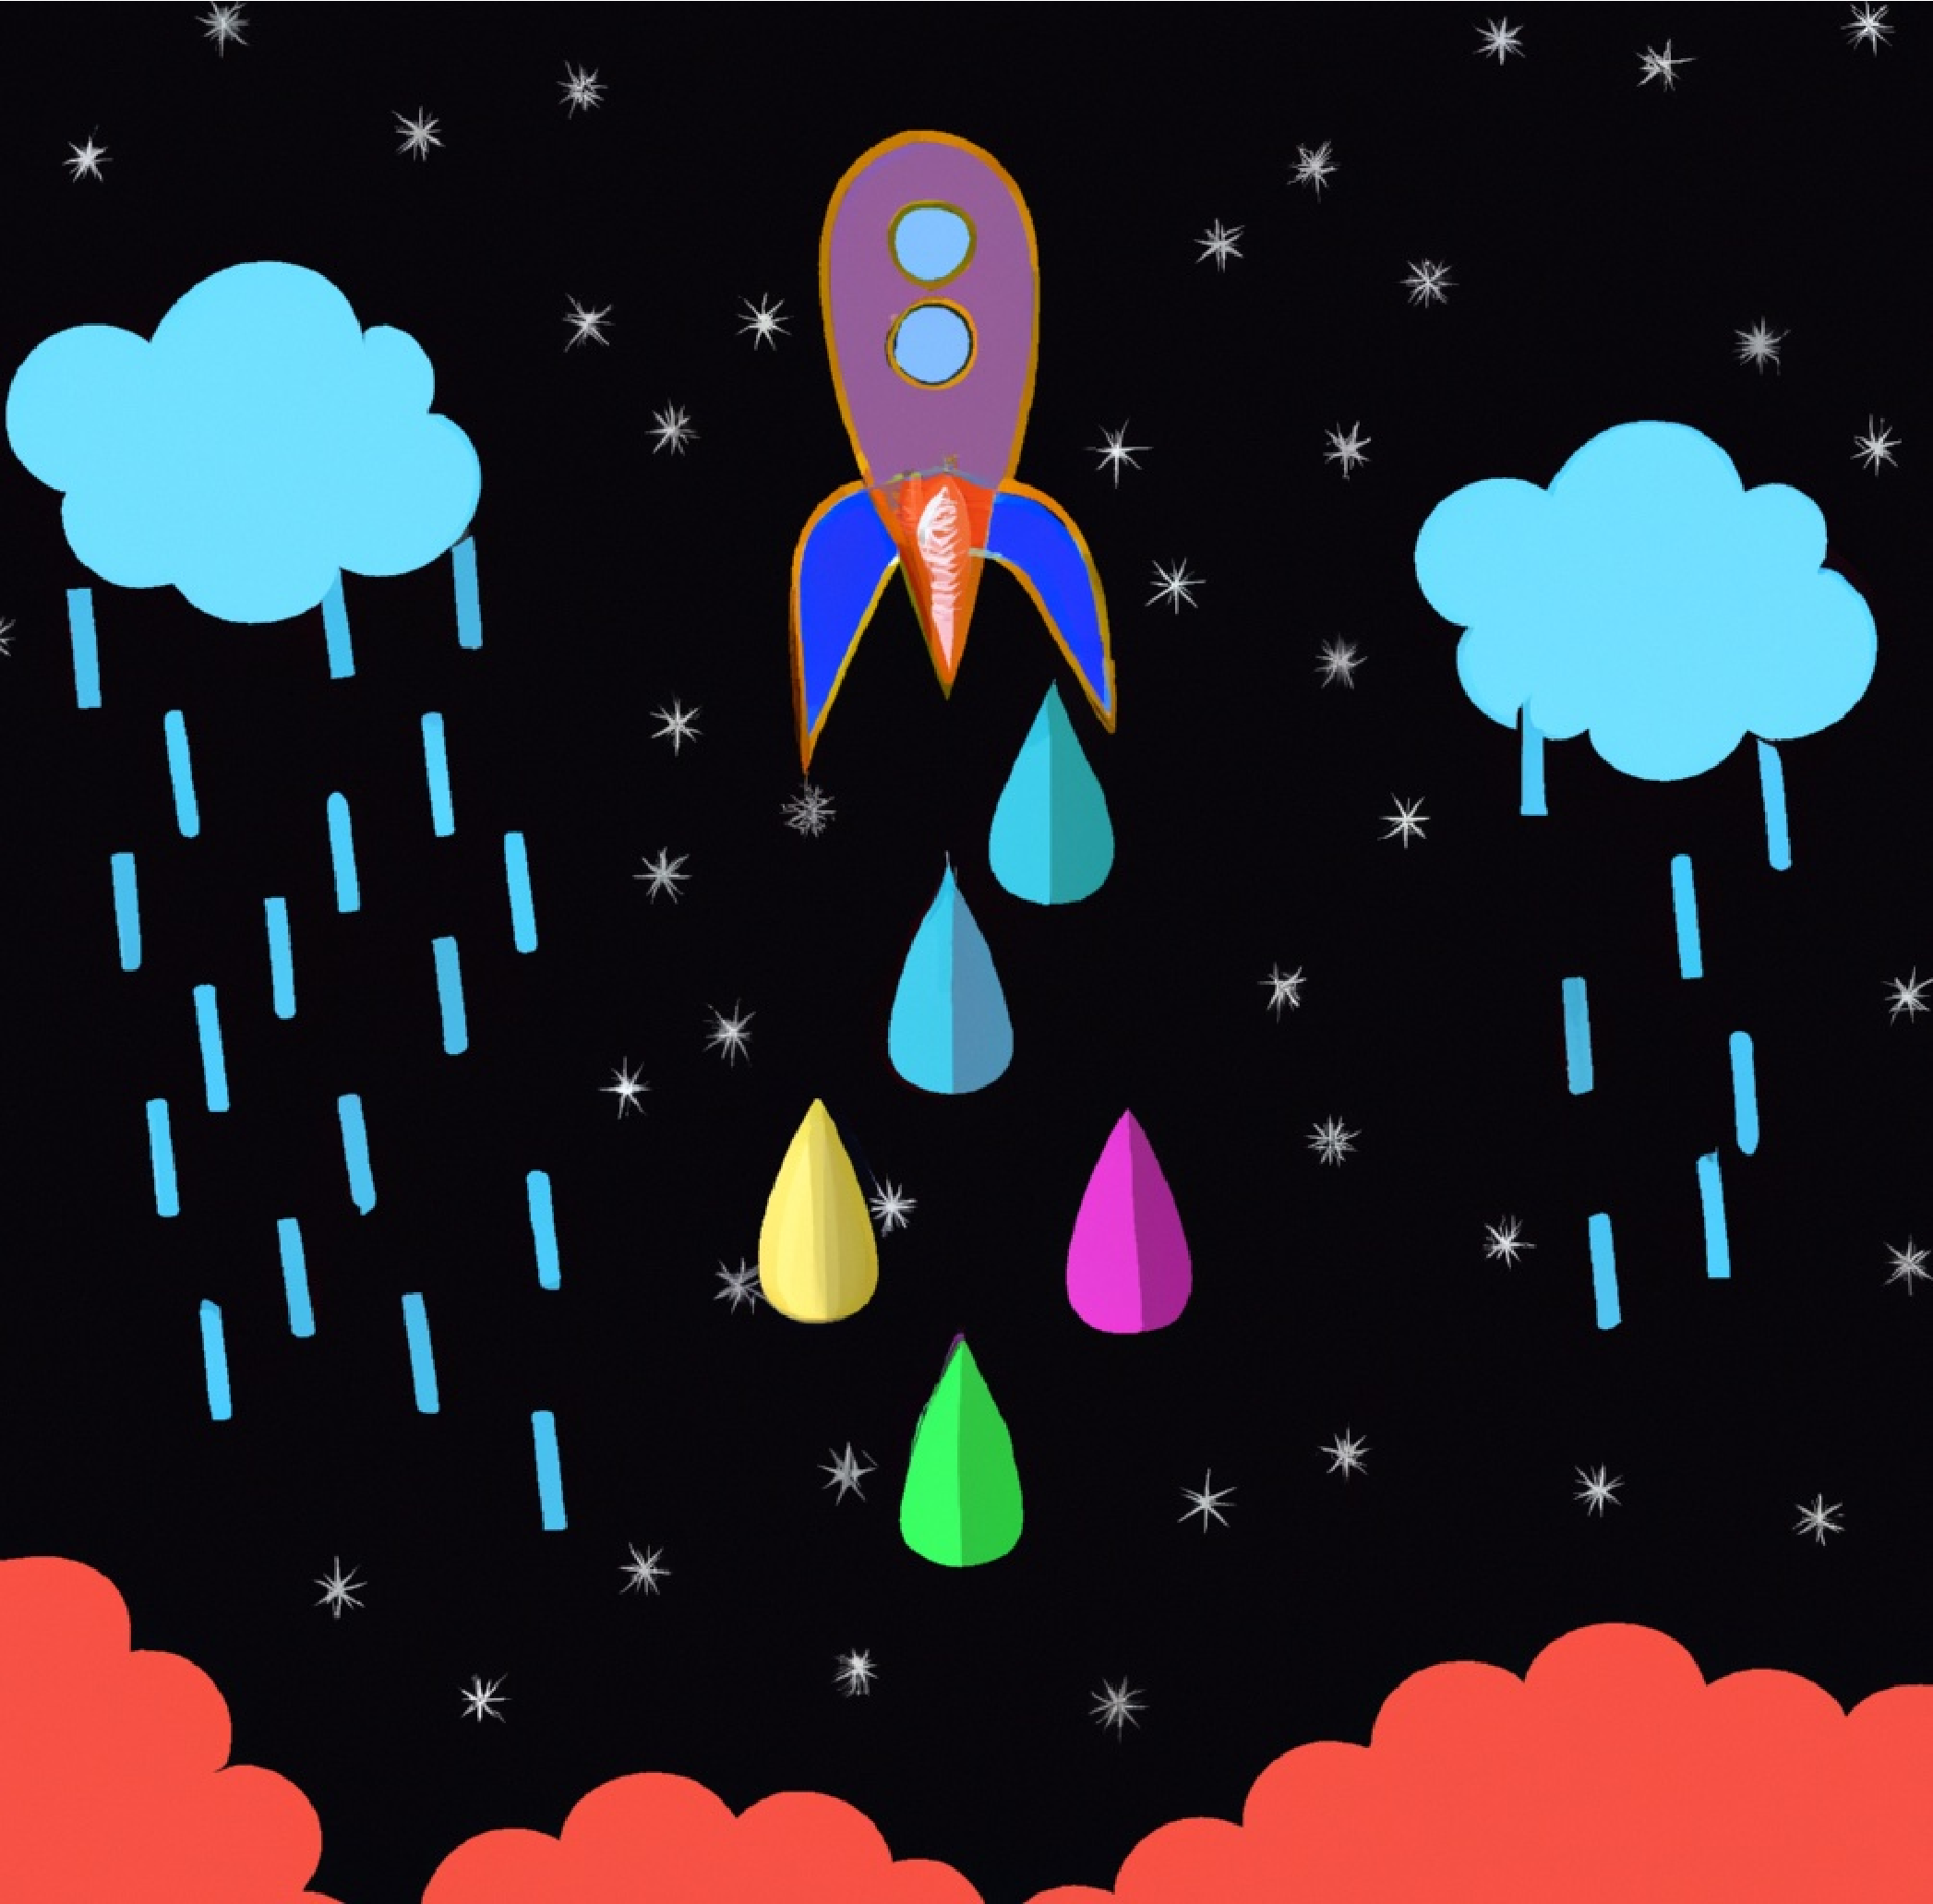
\includegraphics[width=0.36\textwidth]{images/rocketscience.pdf}
    \caption{Caption of the single-image figure \cite{Name2023JCP}}
    \label{fig:single}
\end{figure}

\begin{figure}[t]
    \centering
    \subcaptionbox{First sub-image}{%
        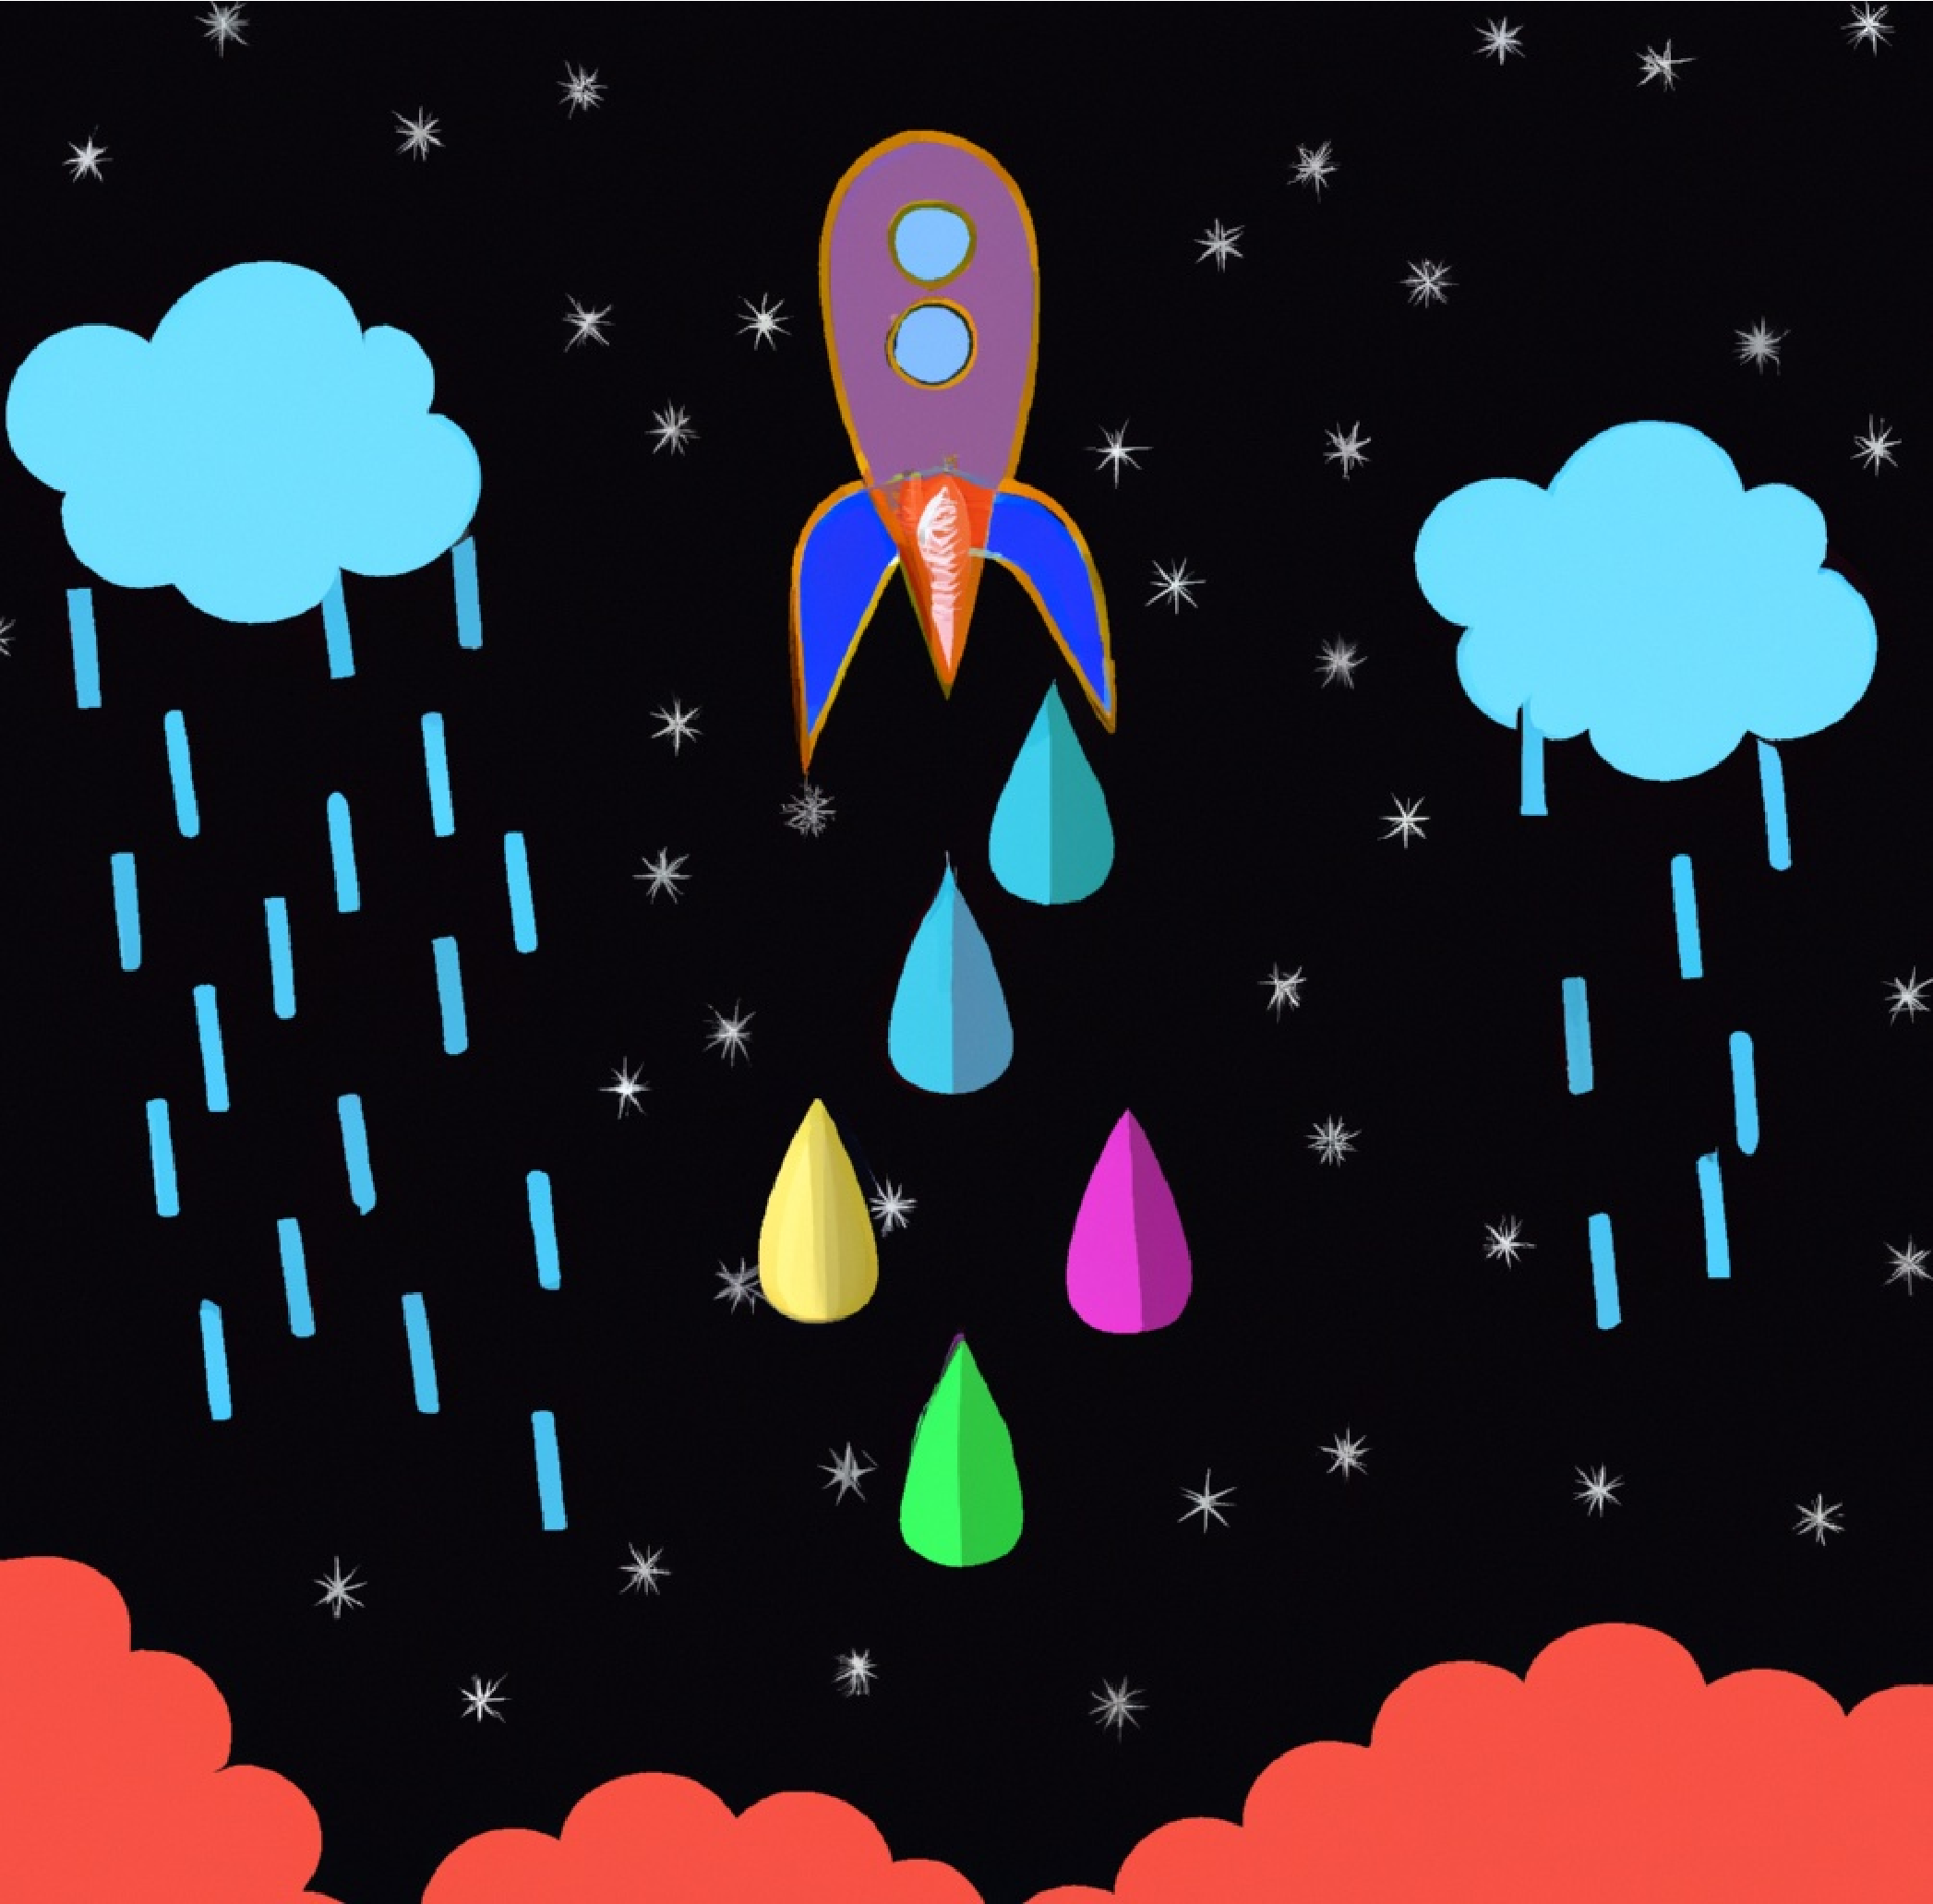
\includegraphics[width=0.32\textwidth]{images/rocketscience.pdf}
    }
    \subcaptionbox{Second sub-image}{%
        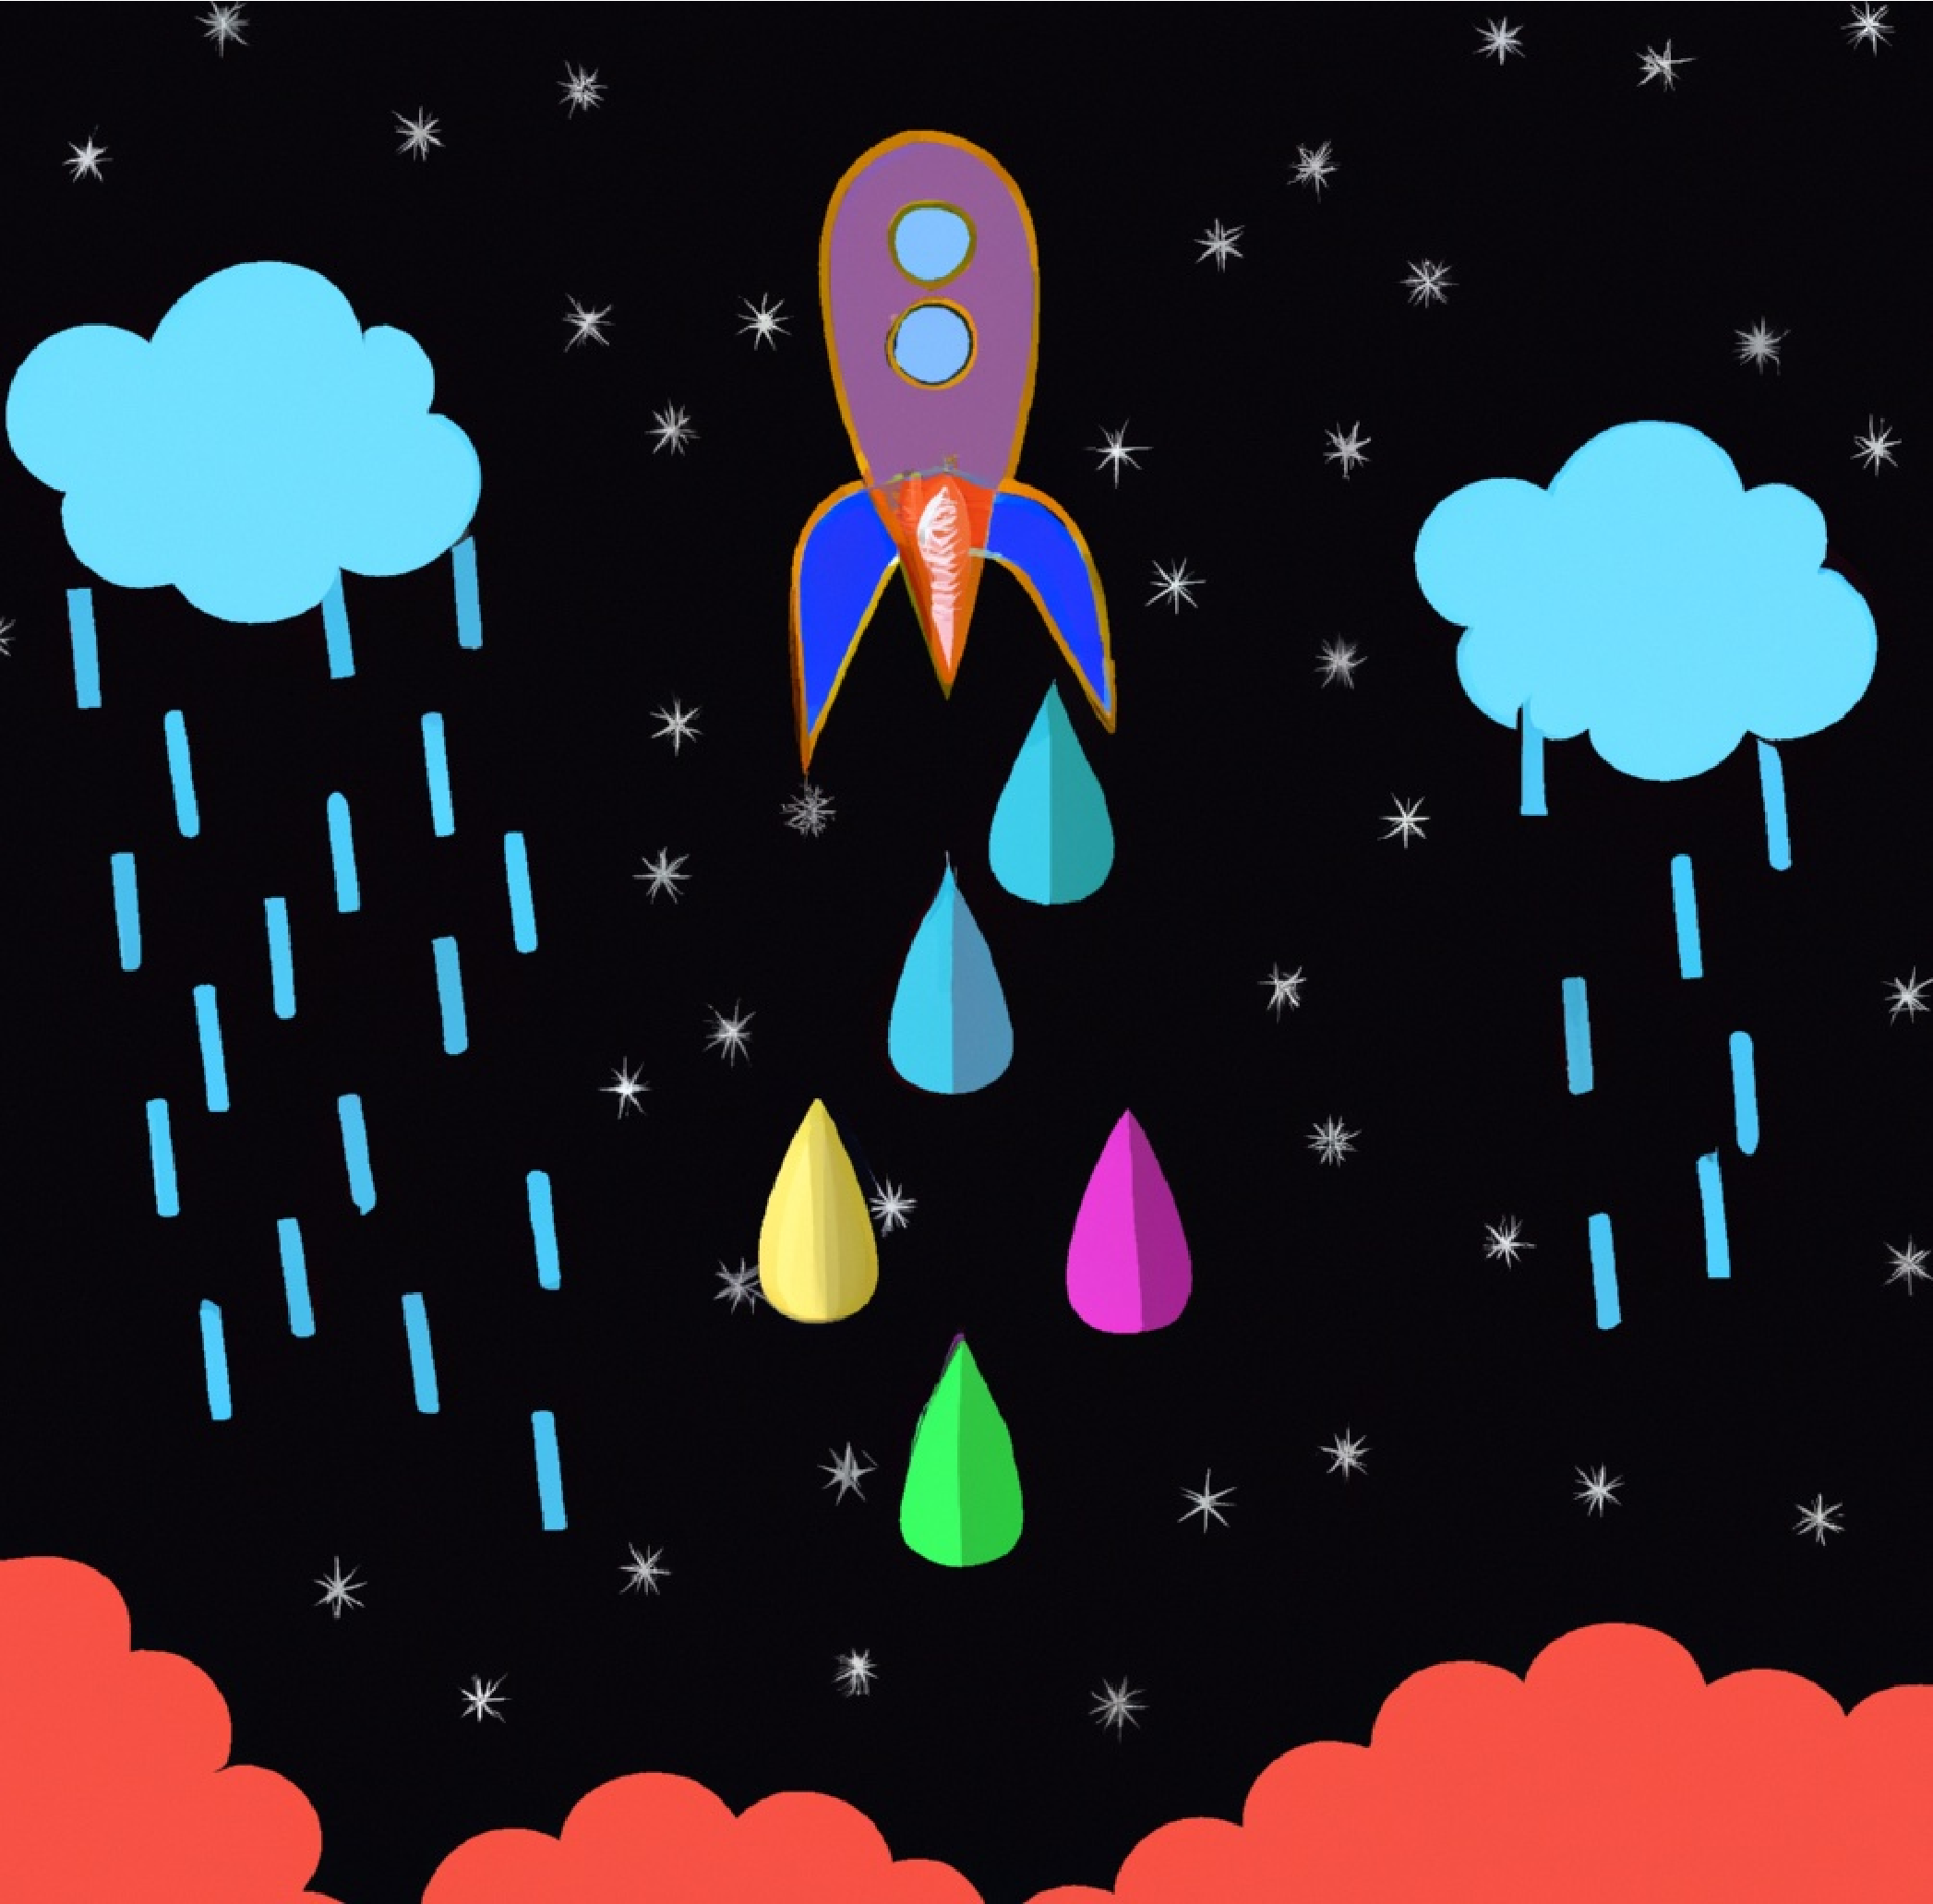
\includegraphics[width=0.32\textwidth]{images/rocketscience.pdf}
    }
    \subcaptionbox{Third sub-image}{%
        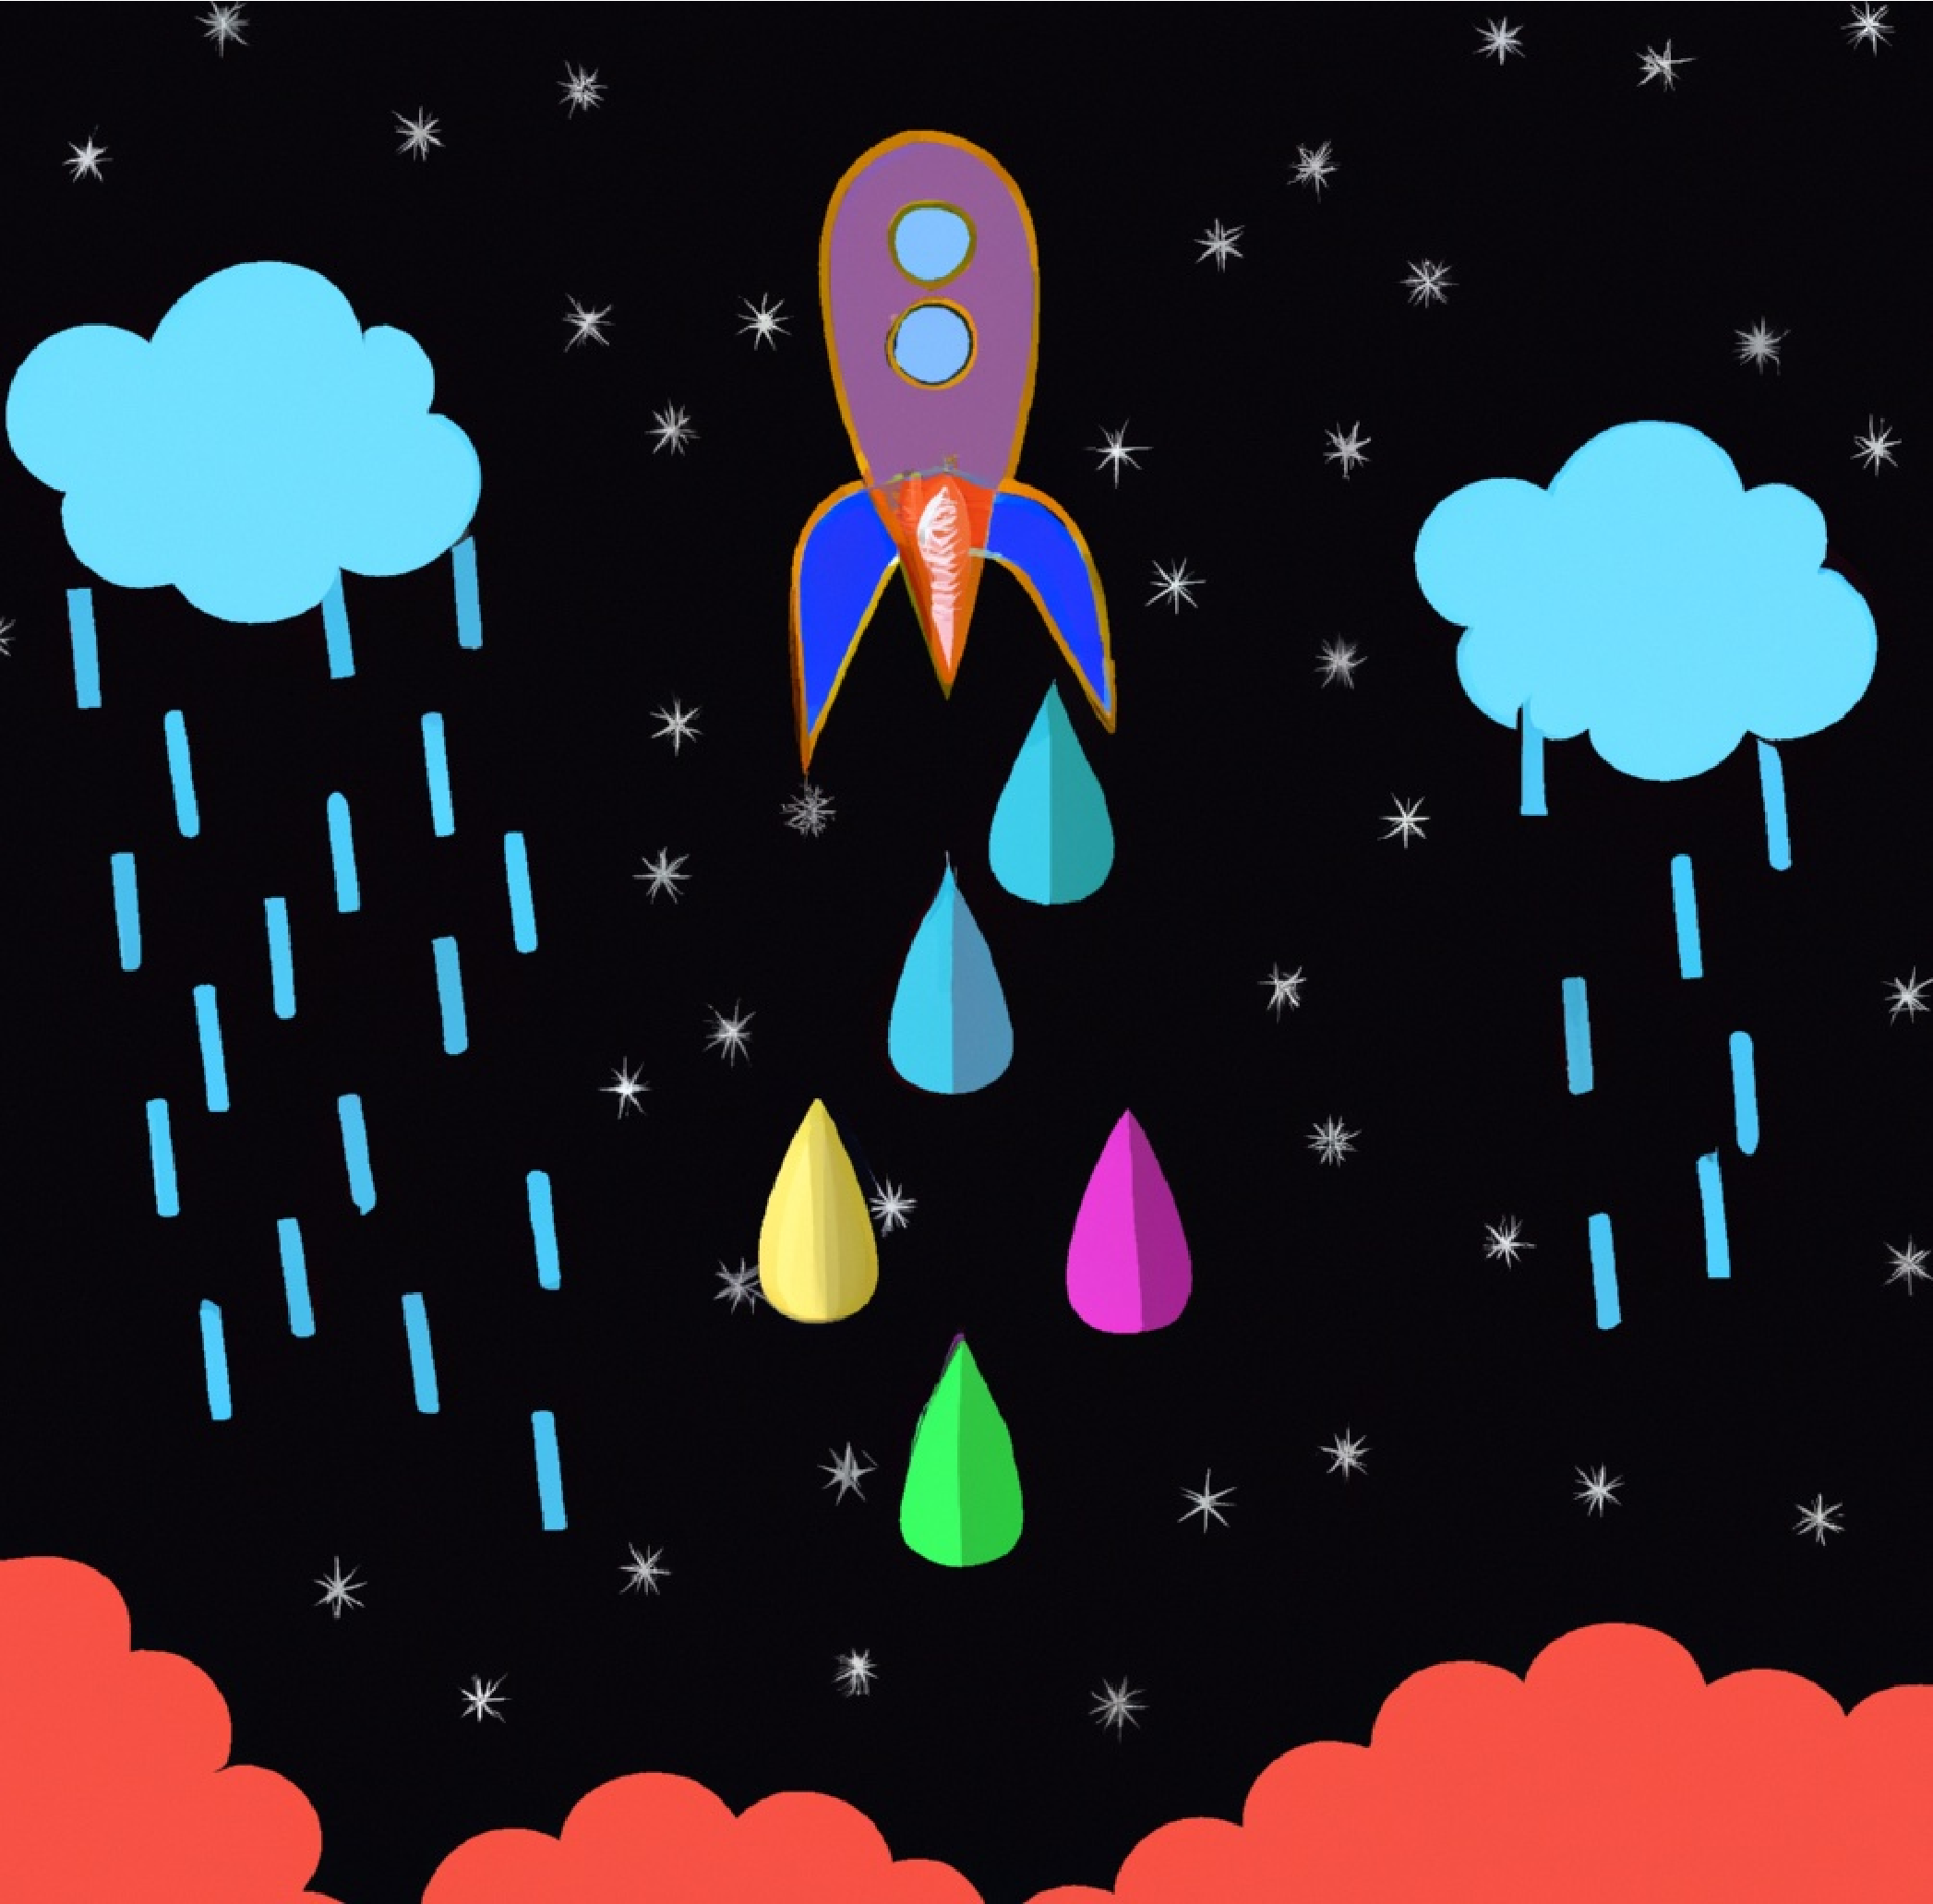
\includegraphics[width=0.32\textwidth]{images/rocketscience.pdf}
    }
    \caption{Caption of the figure of multiple images}
    \label{fig:multiple}
\end{figure}

Figures can be created using the \verb|includegraphics| environment nested inside a \verb|figure| environment, as given in Fig.~\ref{fig:single}. Unlike tables, it is required to use the center alignment command (\verb|\centering|) before the \verb|includegraphics| environment, and the table caption command (\verb|\caption|) after the \verb|includegraphics| command as directed in the style guidelines. It is recommended to place images in subfolders, such as \verb|./images/|, to organize files. Placing images in the root folder is not a good idea. You may also use the \verb|\subcaptionbox| command to place multiple images in a figure, as given in Fig.~\ref{fig:multiple}.

\section{Abbreviations, Symbols, and Glossaries}

\subsection{Use of Abbreviations}

The \verb|\gls{key}| command can be used to automate the use and expansion of abbreviations, when a full definition of the \verb|key| is defined in the \verb|abbrev.tex| file, using the \verb|\newacronym{key}{short}{long}| command. It provides a full definition for the first usage of the acronym in the text. After the initial appearance, the same \verb|\gls| command will only print the acronym. For example, the first time we use \verb|\gls{cfd}| in the text will show \gls{cfd}. Any subsequent uses of \verb|\gls{cfd}| will show only \gls{cfd} since the full definition has already been provided earlier in the text. This feature can save writing effort and improve readability by avoiding the repetition of lengthy phrases. All acronym definitions should be stored in the \verb|abbrev.tex| file.

\subsection{Use of Symbols}

The same \verb|\gls{key}| command can be used to print symbol in the text, when a full definition of the \verb|key| is defined in the \verb|symb.tex| file. The full definition of the symbol can be defined with the \verb|\newsymb{key}{math}{desc}| command.

For example, we can define variables used in an equation, given as:
\begin{equation}
    \psi_1 = x_1 + x_2,
\end{equation}
where \verb|\gls{psi1}| is output, \verb|\gls{x1}| is the first input, and \verb|\gls{x2}| is the second input variables of the system. Then, the definitions given here will read:\\
\noindent where \gls{psi1} is output, \gls{x1} is the first input, and \gls{x2} is the second input variables of the system. Full definitions of all used symbols will appear in the Key to Symbols list in the preliminary pages.

\subsection{Use of Glossaries}

Glossaries can be used with the same \verb|gls{key}| command. Full definition of the term will not appear in the main text, but they will be only defined in the Glossaries section at the end of the document. The full definition of the glossary entry can be defined with the \verb|\newglo{key}{term}{desc}| command, in the \verb|glo.tex| file. For example, here's a sentence using two glossary entries: ``\verb|\Gls{maths}| is important in \verb|\gls{sci}|.'' This sentence will read: ``\Gls{maths} is important in \gls{sci}.''

Command \verb|\Gls| will capitalize the first character. For example, \verb|\Gls{sci}| prints ``\Gls{sci},'' while \verb|\gls{sci}| prints ``\gls{sci}.'' Command \verb|\glspl| will print plural of the term. For example, \verb|\glspl{scientist}| will print ``\glspl{scientist}.''

\subsection{Cross-Referencing Chapters, Tables, Figures, and Equations}

Cross-referencing is possible if entries are numbered and labeled. For example, chapters are all numbered. You may label chapters with \verb|\label{key}| command and refer to the chapter using \verb|\ref{key}| command. For example, since the first chapter is already labeled with \verb|\label{chap:intro}| command, we can refer to this chapter with \verb|Chap.~\ref{chap:intro}| command. It will print as ``Chap.~\ref{chap:intro}.'' Use ``Chapter'' instead of ``Chap.'' only if it is located at the beginning of a sentence. You may also cross-refer other items, including tables and figures. For example, \verb|Tab.~\ref{tab:table-with-long-title}| will print ``Tab.~\ref{tab:table-with-long-title},'' and \verb|Fig.~\ref{fig:single}| will print ``Fig.~\ref{fig:single}.'' You may use ``Table'' and ``Figure'' if they are mentioned at the beginning of a sentence.

Equations are referred using \verb|\eqref{key}| to show parenthesis. For example, \verb|Eq.~\eqref{eq:mtw-signs-subeq}| will print ``Eq.~\eqref{eq:mtw-signs-subeq}.'' If you want to refer to multiple subsequent equations, you may refer the first and last equations, e.g., \verb|Eqs.~\eqref{eq:mtw-sign-subeq1}-\eqref{eq:mtw-sign-subeq3}|. This command will print ``Eqs.~\eqref{eq:mtw-sign-subeq1}-\eqref{eq:mtw-sign-subeq3}.''

With the default \verb|nosecnum| option, sections will not be numbered. In this case, referring section is not possible. If sections need to be referred, consider using \verb|secnum| option with committee approval. With this option, you may label sections and cross-refer them with \verb|Sect.~\ref{sect:labelname}| command.

\listglossaries % Optional. Comment out if glossaries are not used.

\newpage
\bibliographystyle{bibstyle}
\bibliography{ref} % REQUIRED.

\begin{appendix} % Optional. Comment out if appendices are not used.
    \chapter{Chapter Title for the First Appendix}
    
        When you create a chapter within the \verb|appendix| environment, it will be automatically numbered with the prefix "Appendix A," "Appendix B," and so on. You may create as many appendix chapters as needed. The page numbers in the appendix will continue from the last page number of the main text.

    \chapter{Chapter Title for the Second Appendix}

        The appendix typically includes materials that are not essential to the main text but provide additional information or support for the research. Some common examples of content that may go in the appendix include:

        \begin{enumerate}
            \item Raw data: This can include surveys, interviews, or other types of data that were collected during the research process but are too lengthy or detailed to include in the main text.
            \item Supplementary graphs or charts: These can provide additional information or support for the research, but may be too lengthy or detailed to include in the main text.
            \item Technical details: This can include detailed calculations, algorithms, or computer code that are not essential to the main text but may be of interest to readers.
            \item In-depth analysis: This can include detailed statistical analyses or other types of analysis that are not essential to the main text but provide additional support for the research.
            \item Other materials: This can include any other materials that are relevant to the research but are not essential to the main text, such as photographs or illustrations.
        \end{enumerate}
        
\end{appendix}

\end{document}
